\section{Pathway Browser Implementation}
\label{sect:maw_implementation}

\mawappp pathway visualization is relatively simple in terms of its data model;
the \pathcasemaw web service provides all information in terms of graphical
objects such as nodes and edges. \mawapp doesn't need to make any rendering
decisions about an attribute like a node's color based on, for example, a
metabolite's role in a reaction. It simply renders exactly what \pathcasemaw
instructs.

The pathway visualization system was the first part of the project to be
implemented. Its limited scope made it easy to design a graph renderer that is
decoupled from the specific kind of data it displays. Although the design did
have to be modified to be used in \keggapp, the changes were not significant,
and eventually the two applications may share the same code for this component.

Section \ref{sect:smda_arch_overview} describes the general architecture of
\mawappp pathway visualizer. Section \ref{sect:smda_viz_data} describes in
detail the process of loading a graph into memory from its \pathcasemaw
representation. Finally, section \ref{sect:smda_rendering} describes how the
model objects are rendered to the screen.

\subsection{Architecture Overview}
\label{sect:smda_arch_overview}

\begin{figure}[p]
    \center{
        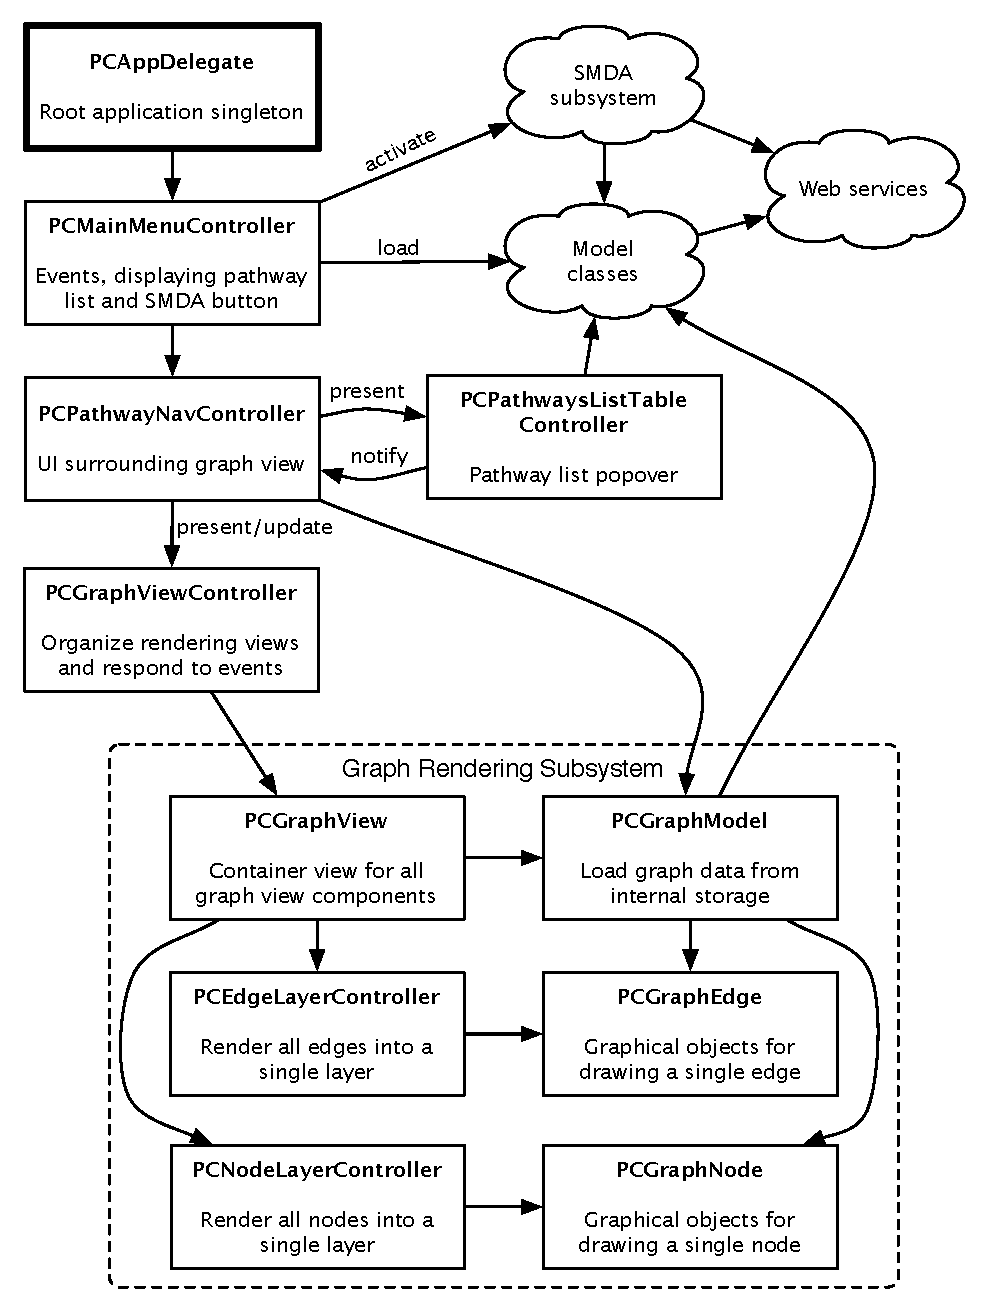
\includegraphics[width=\textwidth]{maw/figures/components.pdf}}
    \caption{\label{fig:maw_components} Components of the architecture. See
    \ref{sect:smda_arch_overview} for more information about this diagram.}
\end{figure}

Figure \ref{fig:maw_components} shows a high-level representation of the
relationships between the most important objects in \mawapp. Most of the classes
discussed here and shown in the figure fall into the category of model, view, or
controller. For more information about Model-View-Controller design, see section
\ref{sect:cocoa_mvc}.

An application-level singleton, \texttt{PCAppDelegate}, handles
application-level delegate methods and notifications from the system. Another
singleton, \texttt{PCMainMenuViewController}, displays the home screen,
including the list of pathways and button to enter SMDA. It also initiates the
download of the model objects if they require an update. This relationship is
represented by the \emph{activates} and \emph{loads} arrows in figure
\ref{fig:maw_components}.

When an item in the list of pathways is tapped, a new view is shown, controlled
by \texttt{PCPathwayNavController}. This view controller object controls the
toolbar and a content area that can contain any view and corresponding view
controller. See the screenshot in figure \ref{fig:maw_screenshot_pathway} to see
how this toolbar is displayed to the user.

The content area is controlled by \texttt{PCGraphViewController}. This view
controller object controls a \texttt{PCGraphView} which renders the pathway
visualization based on a \texttt{PCGraphModel} and sends notifications back to
the \texttt{PCGraphViewController} if an event occurs (e.g. a node being tapped).

As shown in figure \ref{fig:maw_screenshot_pathway_list_popover}, the
``Pathways'' button in the toolbar controlled by \texttt{PCPathwayNavController}
displays a list of pathways that may be visualized. The loading and display of
this list is handled by \texttt{PCPathwayListTableController}, which loads
pathway model objects (\ref{sect:smda_data_model}) and converts them
to a list to be displayed by a table view (\ref{sect:ipad_views}). When a table
view row is selected, the \texttt{PCPathwayListTableController} sends a
notification back to the \texttt{PCPathwayNavController}, which replaces its
content area with a \texttt{PCGraphViewController} representing the new pathway
to be displayed.

The control flow of \texttt{PCPathwayNavController} at runtime is shown in
figure \ref{fig:maw_controlflow}. This object has no event loop of its own; its
functionality is invoked by the application event loop provided by the Cocoa
framework. When the ``Pathways'' button is pressed, it creates a
\texttt{PCPathwayListTableController} which presents a popover containing a
table view, loads the list of pathways, populates the table view, and sends
control back to the event loop. When a row is tapped in this table view, the
\texttt{PCPathwayListTableController} sends a notification back to the
\texttt{PCPathwayNavController}, which hides the popover, loads the new pathway
visualization, and displays it.

\begin{figure}[thbp]
    \center{
        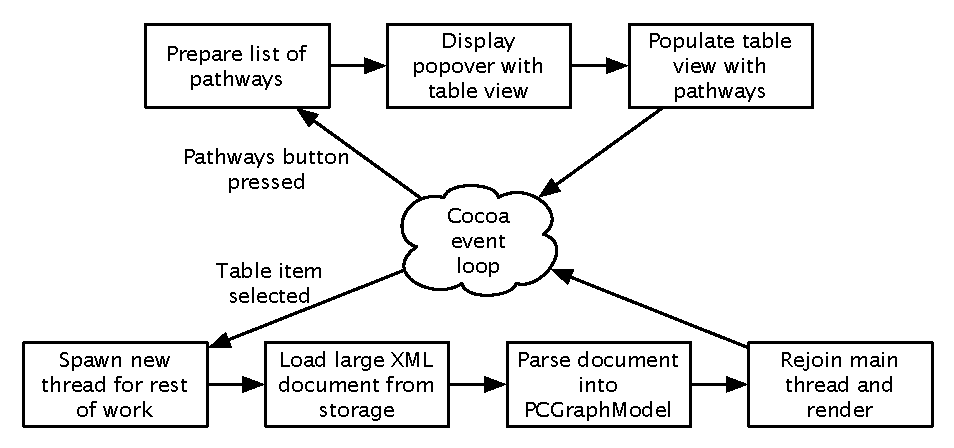
\includegraphics[width=5in]{maw/figures/controlflow.pdf}}
    \caption{\label{fig:maw_controlflow} Control flow of
    \texttt{PCPathwayNavController}}
\end{figure}

\texttt{PCGraphViewController} and \texttt{PCGraphModel} are the high level
interface to the pathway visualization subsystem. \texttt{PCGraphModel} holds
collections (hash tables) of \texttt{PCGraphNode} and \texttt{PCGraphEdge}
objects. These objects represent the visual properties of each node and edge in
the graph, including location, color, shape, label text, and label position. The
\texttt{PCGraphViewController} and its helper objects render the graph
represented by the \texttt{PCGraphModel} to a scroll view
that the user can navigate by touch (\ref{sect:ipad_views}). 

\subsection{Loading Graph Data}
\label{sect:smda_viz_data}

\begin{figure}[thbp]
    \center{
        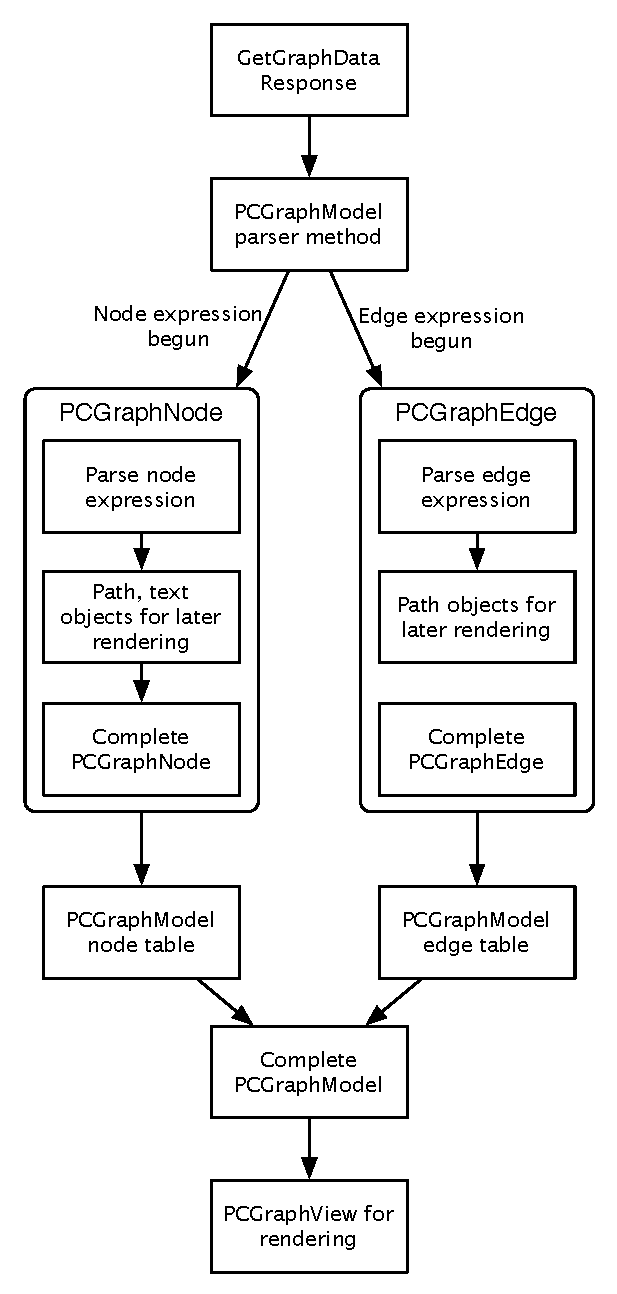
\includegraphics[width=3.5in]{maw/figures/dataflow.pdf}}
    \caption{\label{fig:maw_viz_data} Data flow from \pathcasemaw representation
    to final display format. See \ref{sect:smda_viz_data} for more information
    about this diagram.}
\end{figure}

\subsection{Rendering}
\label{sect:smda_rendering}
